\chapter{METODOLOGI}
Penelitian ini dilakukan sesuai dengan desain sistem berikut beserta implementasinya. Desain sistem adalah konsep dari pembuatan dan perancangan infrastruktur dan kemudian diwujudkan dalam bentuk alur yang harus dikerjakan
% Ubah konten-konten berikut sesuai dengan isi dari metodologi

\section{Metode Penelitian}
Metode penelitian yang akan digunakan pada penelitian ini adalah penelitian pengembangan dari Richey dan Klein\cite{Sugiyono2019}. Metode ini memiliki tiga tahapan yaitu \emph{planning}, \emph{production}, dan \emph{evaluation}. Berikut adalah diagram dari metode yang akan digunakan dalam penelitian ini.
\begin{figure} [H] \centering
  % Nama dari file gambar yang diinputkan
  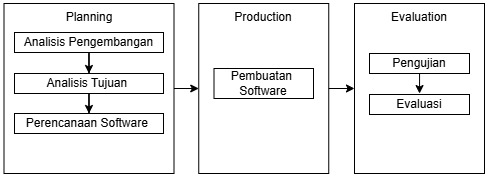
\includegraphics[scale=0.6]{gambar/metodologi penelitian.jpg}
  % Keterangan gambar yang diinputkan
  \caption{Diagram alur penelitian}
  % Label referensi dari gambar yang diinputkan
  \label{fig:Metode penelitian }
\end{figure}
\subsection{Perencanaan(Planning)}
Pada bagian perencanaan, peneliti melakukan analisis pengembangan terhadpat kursi roda yang sudah ada sebelumnya. Analisis pengembangan ini diperlukan agar penilit dapat mengetahui hal apa yang bisa dikembang dari kursi roda. Berdasarkan hasil dari analisis pengembangan, hal yang dapat dikembangkan dari kursi roda adalah bagian \emph{software}.
\subsection{Produksi(Production)}
Tahan produksi meliputi pembuatan dari \emph{software} dari kursi roda berdasarkan dari perencanaan software dan analisis tujuan yang telah ditentukan di tahan \emph{planning}.
\subsection{Evaluasi(Evaluation)}
Pada tahap ini, dilakukan pengujian secara bertahap untuk memastikan kursi roda dapat beroperasi sesuai dengan tujuan yang telah ditetapkan.

\section{Analisis sistem}
Sebelum memulai pengembangan sistem, penting untuk melakukan analisis terhadap sistem.
Analisis ini diperlukan untuk mengetahui kebutuhan dan tujuan yang ingin dicapai. Tujuan dari analisis kebutuhan adalah identifikasi berbagai elemen yang diperlukan untuk sistem, baik dari sudut pandang fungsional maupun non-fungsional. Untuk memastikan bahwa sistem yang dikembangkan memenuhi persyaratan perlu ditetapkan spesifikasi dan persyaratan.

\subsection{Analisis Kebutuhan}
Analisis kebutuhan dilakukan dengan mengumpulkan data dari studi literatur terkait. Analisis ini bertujuan untuk mengidentifikasi fitur-fitur dan spesifikasi teknis yang diperlukan dalam pengembangan sistem. Berdasarkan hasil analisis, beberapa
kebutuhan sistem yang harus dipenuhi adalah sebagai berikut:
\begin{enumerate}
    \item Penggunaan gesture SIBI sebagai metode utama kendali kursi roda cerdas.
    \item Penelitian pada penggunaan LSTM untuk pengenalan dan deteksi gesture tangan SIBI yang dikombinasikan dengan perangkat keras seperti kamera.
    \item Penggunaan LSTM pada pemrosesan urutan data gesture yang diambil dari kamera.
    \item Pengembangan smart braking system untuk meningkatkan keselamatan pengguna kursi roda dalam mendeteksi objek di sekitar kursi roda dan melakukan pengereman otomatis. 
    \item Sistem smart breaking ini akan berfungsi untuk mendeteksi manusia dan objek lain di lingkungan sekitarnya.
    \item Penelitian difokuskan pada pengembangan dan integrasi antara perangkat keras (kamera, motor kursi roda) dan perangkat lunak kontrol kursi roda dan smart braking system.
    \item Pengontrol kursi roda akan diimplementasikan untuk memberikan respon sesuai dengan gestur yang dipanggil dan berhenti otomatis ketika mendeteksi manusia di depannya.
\end{enumerate}
\subsection{Analisis Tujuan}
Berdasarkan hasil analisis kebutuhan, tujuan pengembangan dari sistem ini ditetapkan untuk
memastikan bahwa sistem yang dikembangkan dapat memenuhi spesifikasi dan operasional
yang diperlukan. Adapun tujuan dari ingin dicapai dalam pengembangan sistem ini adalah:
\begin{enumerate}
    \item Membuat sebuah sistem untuk mendeteksi gestur SIBI menggunakan LSTM.
    \item Membuat sebuah sistem untuk mendeteksi objek menggunakan YOLOv11 untuk sistem pengereman otomatis.
\end{enumerate}

\section{Rancangan Penelitian}
\begin{figure} [H] \centering
  % Nama dari file gambar yang diinputkan
  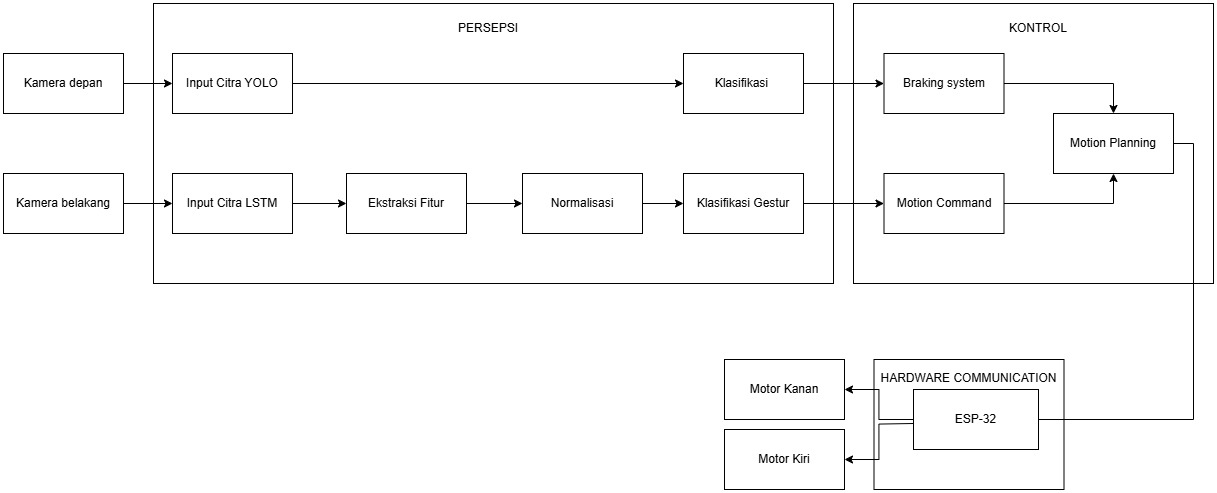
\includegraphics[scale=0.4]{gambar/rancangan penelitian.jpg}
  % Keterangan gambar yang diinputkan
  \caption{Blok diagram dari sistem}
  % Label referensi dari gambar yang diinputkan
  \label{fig:rancangan penelitian}
\end{figure}
Pada tahap ini, sistem akan diterapkan sesuai dengan desain dan implementasi yang telah direncanakan sebelumnya. Diagram ini mencakup dari pengembangan software, alur sistem, dan implementasi infrastruktur. 
\section{Software}
\begin{figure} [H] \centering
  % Nama dari file gambar yang diinputkan
  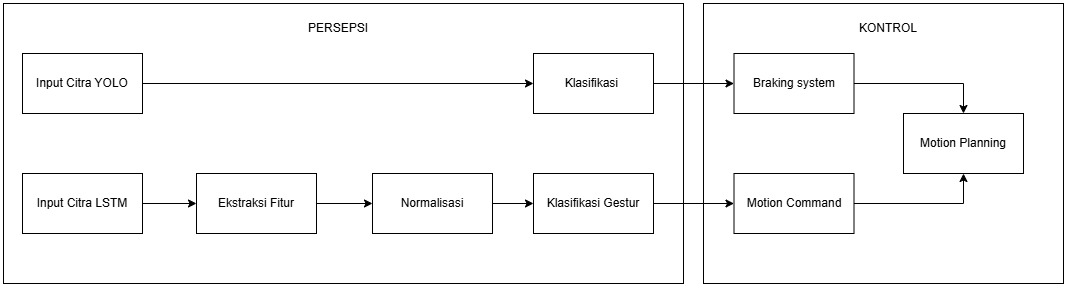
\includegraphics[scale=0.4]{gambar/software new.jpg}
  % Keterangan gambar yang diinputkan
  \caption{Diagram dari \emph{software}}
  % Label referensi dari gambar yang diinputkan
  \label{fig:diagram software}
\end{figure}
Pada tahap ini, merupakan pembuatan dari software yang telah ditentukan pada perencanaan \emph{software}. Gambar 3.2 merupakan blok diagram dari alur yang akan dijelaskan sebagai berikut:

\subsection{Input Citra YOLO}
Input untuk YOLO biasanya berupa citra dalam format digital (misalnya JPG atau PNG) yang telah diubah ukurannya sesuai dengan kebutuhan model. Sebelum dimasukkan ke model, citra tersebut dinormalisasi, yaitu nilai pikselnya diubah menjadi rentang 0 hingga 1 untuk mempercepat proses komputasi. YOLO membagi citra menjadi grid, di mana setiap grid bertanggung jawab untuk memprediksi bounding box, confidence score, dan kelas objek di dalam grid tersebut. Proses ini menghasilkan output berupa koordinat bounding box, skor probabilitas, dan label kelas untuk setiap objek yang terdeteksi.

\subsection{Labelling menggunakan Roboflow}
Input citra yang didaptkan tadi lalu akan dilabeli dan diaugmentasi. Dimana Roboflow digunakan untuk melakukan proses labeli dan augmentasi ini. Roboflow memiliki tools yang mumpuni dalam melakukan labeling. Dimana terdapat beberapa proses yang akan dilakukan yaitu, import dataset, pelabelan dataset dan augmentasi dataset.

\begin{figure} [H] \centering
  % Nama dari file gambar yang diinputkan
  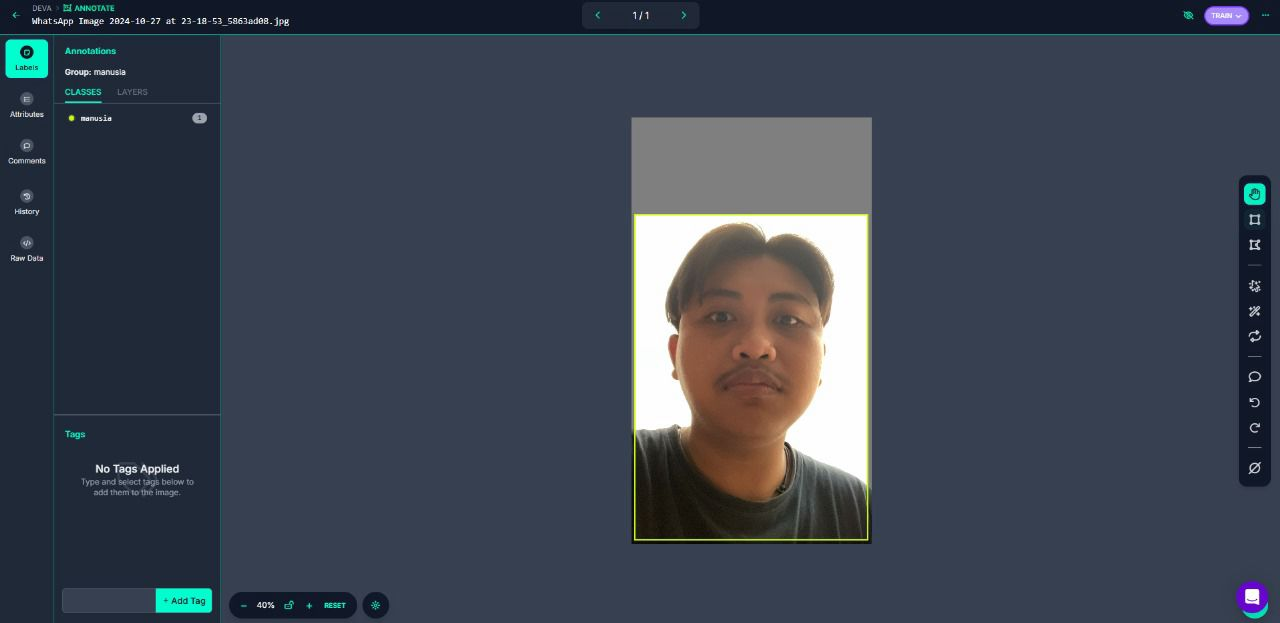
\includegraphics[scale=0.2]{gambar/devafoto.jpeg}
  % Keterangan gambar yang diinputkan
  \caption{Labeling pada Roboflow}
  % Label referensi dari gambar yang diinputkan
  \label{fig:rancangan penelitian}
\end{figure}

Dalam Proses anotasi penamaan class yang digunakan haruslah sesuai dengan objek yang akan dideteksi. Dalam Konteksi tugas akhir kali ini objek yang akan dideteksi adalah manusia. Maka digunakanlah nama manusia sebagai penamaan dari kelas yang akan digunakan. Adapun dalam proses anotasi harus diperhatikan objek yang akan dianotasikan harus sesuai agar tidak ada kesalahan model dalam mendeteksi. %Setelah selesai maka dataset akan terlihat seperti gambar dibawah. 

setelah seluruh gambar yang dipilih telah dianotasi. Maka disimpan dalam bentuk versi yang mudah diingat, apabila terjadi perubahan pada dataset maka akan disimpan dalam versi lain.

%Adapun fitur pemberian augmentasi pada dataset yang merupakan tools dari roboflow yang berguna untuk memberikan variasi dari dataset, gambar berikut adalah contoh pemberian augmentasi dataset. Setelah selesai pemberian augmentasi maka dataset ini sudah dapat digunakan untuk dilakukan klasifikasi menggunakan YOLOV8, YOLOV11 dan YOLOV12.

\subsection{Klasifikasi}
Klasifikasi dalam YOLO (You Only Look Once) adalah proses di mana model menentukan kategori atau kelas dari objek yang terdeteksi dalam sebuah citra. Setelah model YOLO mendeteksi keberadaan objek melalui bounding box, langkah berikutnya adalah mengklasifikasikan objek tersebut ke dalam salah satu kelas yang telah dilatih, seperti mobil, orang, hewan, atau benda lainnya, dalam penelitian kelas yang digunakan adalah manusia.

%Proses ini melibatkan softmax function atau sigmoid activation (tergantung pada versi YOLO) untuk menghasilkan probabilitas dari setiap kelas. Probabilitas ini menunjukkan keyakinan model bahwa objek dalam bounding box tersebut termasuk ke dalam kelas tertentu. Kelas dengan probabilitas tertinggi dipilih sebagai hasil klasifikasi. Kombinasi antara deteksi (bounding box) dan klasifikasi memungkinkan YOLO untuk mengenali posisi serta jenis objek dalam sebuah citra secara simultan.

\subsection{Klasifikasi YOLOV8}
Klasifikasi dilakukan setelah melakukan proses labelling yang akan dikenali menggunakan YOLOV8 yang telah ditraining untuk mengenali manusia yang terdapat pada citra. Model akan memberikan output berupa kelas yaitu manusia, nantinya hasil dari klasifikasi akan dijadikan acuan untuk melakukan \emph{braking}.

Model yang digunakan memiliki output kelas berupa manusia, adapun hasilnya berupa \emph{bounding box} pada manusia yang terdeteksi. Adapun arsitektur yang digunakan pada YOLOV8 

\begin{figure} [H] \centering
  % Nama dari file gambar yang diinputkan
  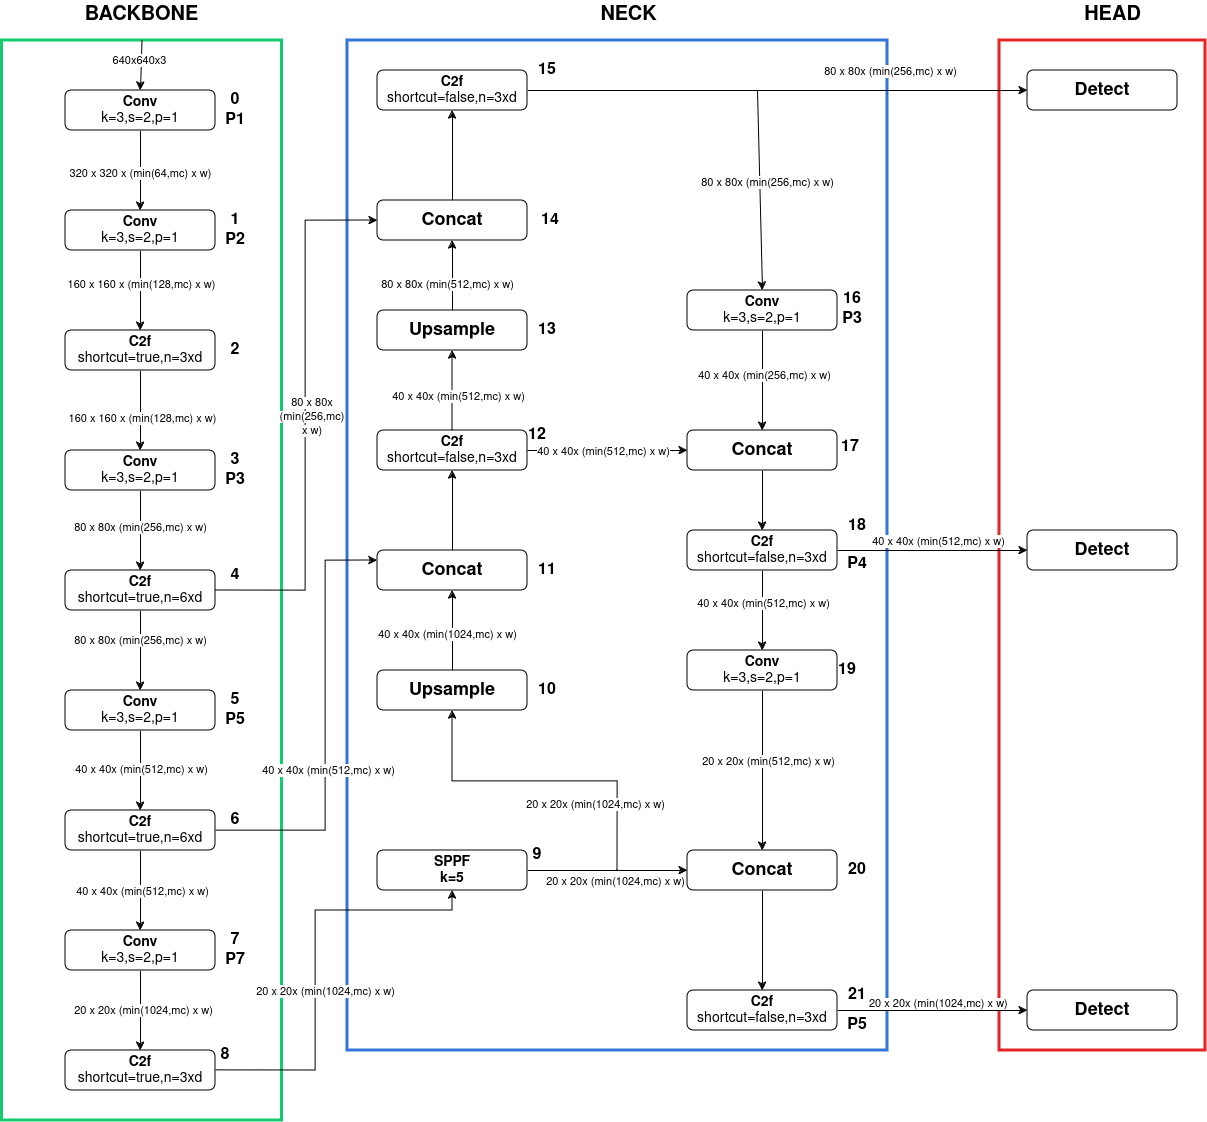
\includegraphics[scale=0.3]{gambar/yolov8.png}
  % Keterangan gambar yang diinputkan
  \caption{Blok diagram dari sistem}
  % Label referensi dari gambar yang diinputkan
  \label{fig:rancangan penelitian}
\end{figure}

Arsitektur YOLOV8 menggunakan \emph{convolutional neural network (CNN)} sebagai dasar dalam YOLO, jaringan CNN digunakan untuk ekstraksi fitur dari gambar yang telah diinputkan dan kemudian menerapkan jaringan lain untuk memprediksi bounding box dan kelas objek langsung dari gambar tersebut. Adapun selain lapisan CNN terdapat juga lapisan Concat, lapisan Upsampling, Blok SPPF, Blok C2f.

Adapun dalam arsitektur YOLOV8 dibagi menjadi bagian backbone, neck dan head. agar dapat memahami arsitektur YOLOV8 akan dibahas satu per satu fungsi dari lapisan dan blok yang digunakan pada YOLOV8. Lapisan Convolution (Conv) fungsinya yaitu melakukan operasi convolusi pada gambar input untuk mengekstraksi fitur pada gambar. operasi ini melibatkan filter pada gambar, mengkalikan dan menjumlahkan nilai nilai piksel untuk menghasilkan fitur map baru.

Blok C2f atau yang sering disebut dengan Cross Stage Spatial Network, dimana pada blok ini digabungka beberapa lapisan convolusi dengan skip connection, yang meningkatkan pemahaman konteks spasial dan fitur kompleks

Blok SPPF (spatial pyramid pooling fast) bertujuan untuk menangkap dari bebagai skala fitur map dengan menerapkan pooling pada beberapa tingkat. Sebagai contoh 1x1, 3x3 dan 5x5.

Lapisan Upsampling meningkatkan resolusi fitur map dengan memperbesar dimensinya menggunakan metode seperti neaarest neighbor atau bilinear interpolation, memungkinkan deteksi objek dengan resolusi yang lebih tinggi

Lapisan Concat (concatenate) menggabungkan dua atau lebih fitur map dari jalur berbeda dalam model. ini dilakukan dengan menggabungkan fitur map di sepanjang dimensi channel, sehingga mempertahankan  informasi dari berbagai tahap pemrosesan sebelumnya sehingga menghasilkan konteks yang lebih kaya untuk deteksi objek.

\subsection{Klasifikasi YOLOV11}
Klasifikasi pada YOLOV11 juga menggunakan data yang sudah dilabeling pada proses sebelumnya. Dimana output yang diharapkan dari training yaitu berupa kelas yaitu manusia.

YOLOV11 menggunakan arsitektur yang kurang lebih sama dengan YOLOV8 dengan perubahan pada Blok C2f yang diganti dengan Blok C3K2 yang merupakan upgrade untuk menghasilkan deteksi yang lebih baik dan lebih effisien. adapun arsitektur YOLOV11 sebagai 

\begin{figure} [H] \centering
  % Nama dari file gambar yang diinputkan
  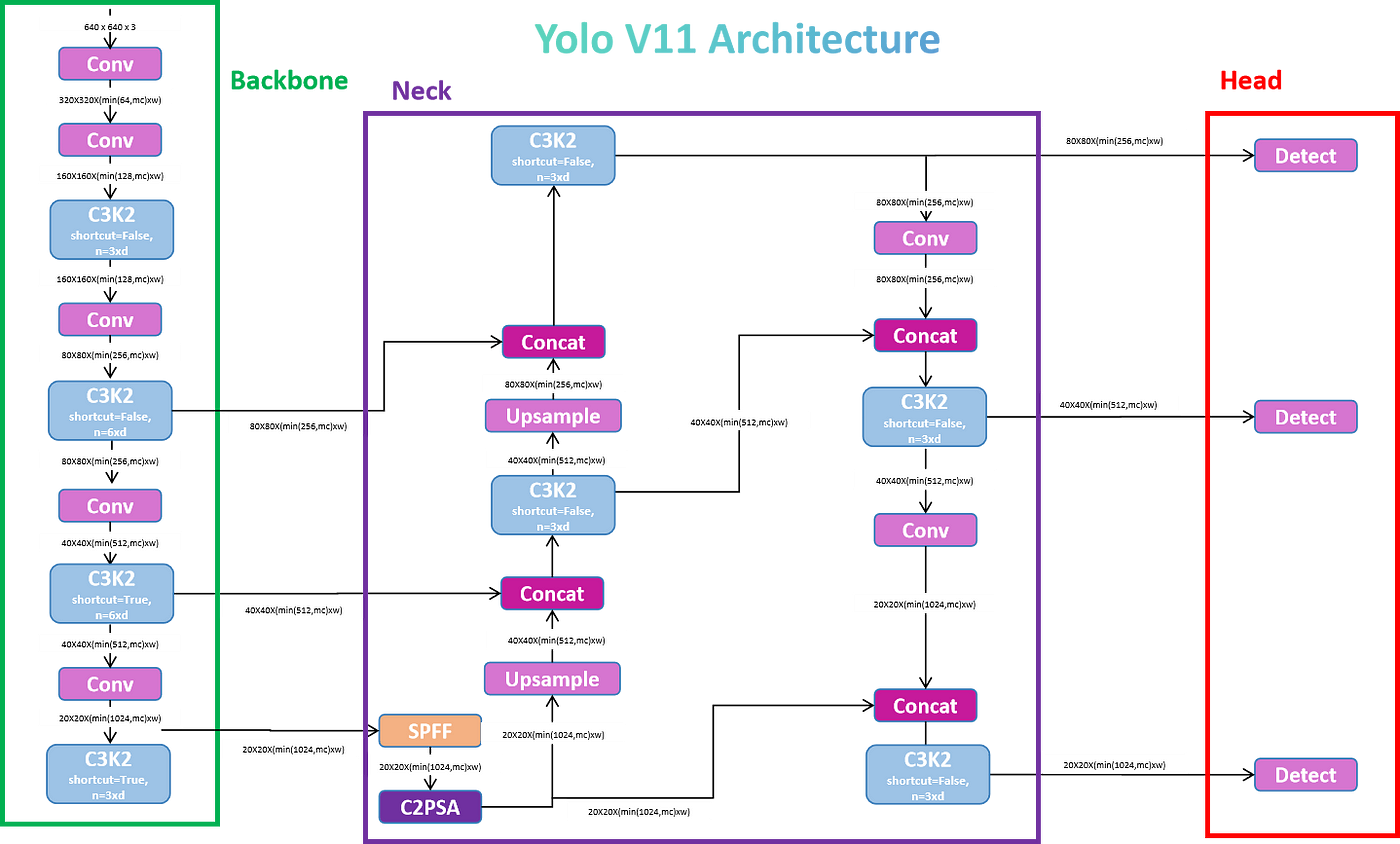
\includegraphics[scale=0.25]{gambar/yolov11.png}
  % Keterangan gambar yang diinputkan
  \caption{Blok diagram dari sistem}
  % Label referensi dari gambar yang diinputkan
  \label{fig:rancangan penelitian}
\end{figure}

Blok C3k2 berisi lapisan convolusi yang digabungkan dengan blok C3K dan lapisan concat. adapun lapisan ini digunakan untuk menghasilkan ekstraksi fitur yang lebih baik, terutama untuk objek yang berukuran kecil. Berikut merupakan isi dari Blok C2f pada YOLOV8 dan C3K2 pada YOLOV11.

\begin{figure} [H] \centering
  % Nama dari file gambar yang diinputkan
  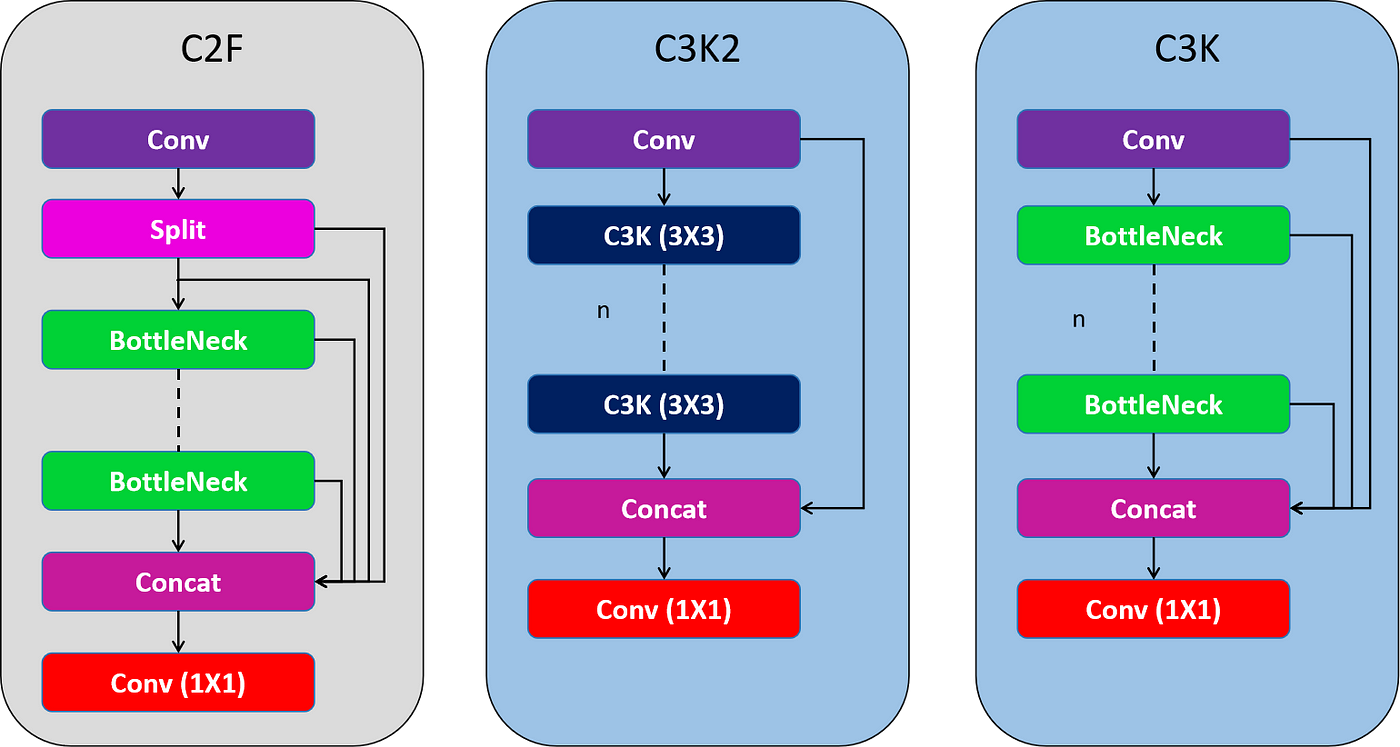
\includegraphics[scale=0.18]{gambar/c2f c3k2.png}
  % Keterangan gambar yang diinputkan
  \caption{Blok diagram dari sistem}
  % Label referensi dari gambar yang diinputkan
  \label{fig:rancangan penelitian}
\end{figure}


\subsection{Klasifikasi YOLOV12}
Klasifikasi pada YOLOV12 juga menggunakan data yang sudah dilabeling pada proses sebelumnya. Dimana output yang diharapkan dari training yaitu berupa kelas yaitu manusia.

YOLOV12 menggunakan arsitektur yang kurang lebih sama dengan YOLOV8 dan YOLOV11 dengan perubahan pada Blok C3K2  yang diganti dengan Blok R ELAN yang merupakan upgrade agar output pembelajaran fitur yang lebih baik dan gradien yang lebih efisien. adapun isi dari blok R ELAN dan perbandingannya dengan blok sebelumnya dapat dilihat sebagai  

\begin{figure} [H] \centering
  % Nama dari file gambar yang diinputkan
  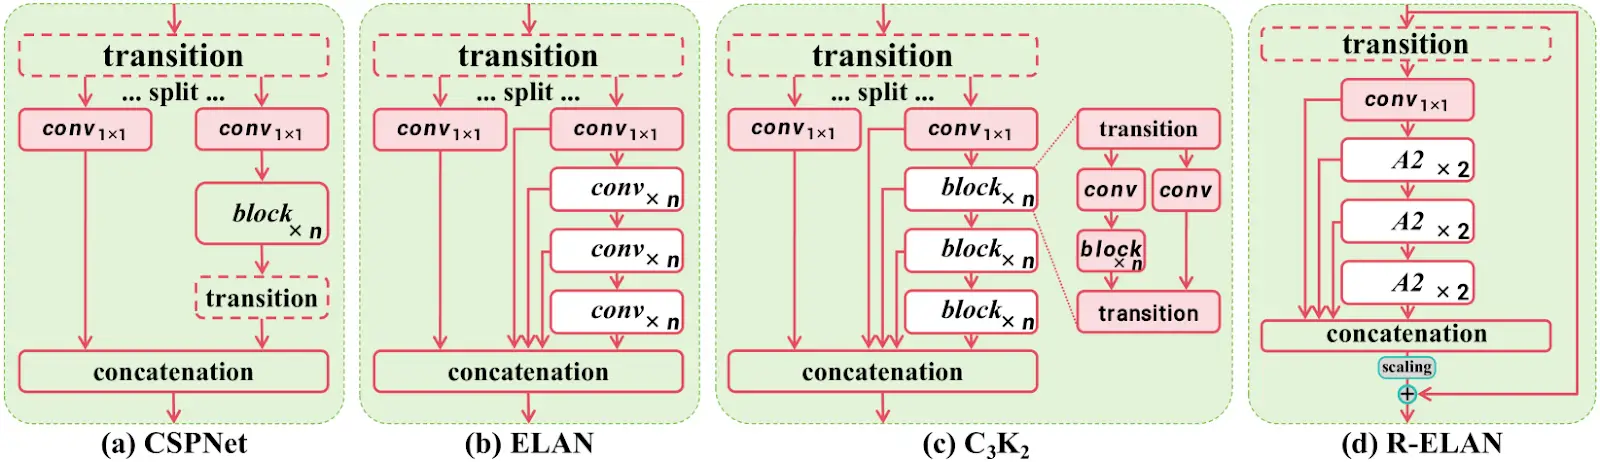
\includegraphics[scale=0.18]{gambar/r elan.png}
  % Keterangan gambar yang diinputkan
  \caption{Blok diagram dari sistem}
  % Label referensi dari gambar yang diinputkan
  \label{fig:rancangan penelitian}
\end{figure}

Blok R ELAN berisi lapisan convolusi (1x1) transition layer yang berfungsi untuk mereduksi input, lalu dilanjutkan dengan split feature map yang digunakan untuk memisahkan fitur ke beberapa bagian, lalu dilanjutkan ke lapisan convolusi (3x3) yang telah di stack untuk mengekstraksi fitur secara mendalam, lalu ada shortcut yang menghubungkan input dan output, dan diakhiri dengan lapisan concat yang menghubungkan semua output tersebut kedalam satu tensor. Dengan penggabungan setiap lapisan tersebut menghasilkan blok yang memiliki fungsi untuk memaksimalkan pemrosesan fitur sambil menjaga stabilitas pelatihan, dengan struktur residual dan strategi agregasi efisien.

\subsection{Preprocessing}
Setelah citra diklasifikasi maka akan dilakukan Preprocessing yang menghasilkan jarak dari citra yang didapatkan. Adapun proses ini melibatkan perhitungan dari nilai nilai yang didapatkan dari bounding box dalam layar, Seperti tinggi bounding box dalam pixel maupun lebar bounding box dalam pixel.

Untuk mendapatkan jarak menggunakan bounding box dengan menerapkan konsep Fokus Panjang dalam Pixel \emph{Focal Length Pixel}. Adapun fokus panjang dalam pixel ini adalah konversi dari fokus panjang lensa kamera  yang biasanya diukur dalam meter ke dalam satuan pixel. Konsep ini biasa digunakan dalam visi komputer untuk menghubungkan informasi visual dari kamera ke ukuran fisik di dunia nyata. Adapun rumus Fokus panjang dalam pixel dapat dilihat pada rumusan berikut

\begin{equation}
    f_p = \frac{D \times h_b}{H-o}
\end{equation}

Dimana :
\begin{itemize}
    \item $f_p$ adalah \emph{focal length pixel}.
    \item $D$ adalah jarak sebenarnya dari kamera ke objek.
    \item $h_b$ adalah tinggi bounding box dalam piksel.
    \item $H_o$ adalah tinggi sebenarnya dalam objek.
\end{itemize}

Dengan mendapatkan nilai $f_p$ kita dapat mengkonversi pengukuran dari ruang gambar (piksel) ke dimensi dunia nyata (meter atau centimeter). Nilai tinggi rata rata manusia juga digunakan untuk melakukan konversi. Adapun rumus konversinya sebagai berikut

\begin{equation}
    D = \frac{f_p \times H_o}{h_b}
\end{equation}

Dimana :
\begin{itemize}
    \item $H_o$ merupakan tinggi rata - rata manusia
\end{itemize}

Jarak yang didapatkan sekarang dapat digunakan dalam sistem braking yang akan diimplementasikan di kursi roda. Dimana pada proyek kali ini digunakan Jarak 1.3 meter sebagai syarat kursi roda untuk berhenti. Yang mana apabila sudah dijarak 1.3 meter maka kursi roda akan berhenti.

\subsection{Input Citra LSTM}
Pada tahap ini, diawali dengan pengambilan citra untuk dataset. Pengambilan dataset dilakukan langsung melalui kursi roda dengan menggunakan kamera yang menghadap ke pengguna kursi roda. 
\begin{figure} [H] \centering
  % Nama dari file gambar yang diinputkan
  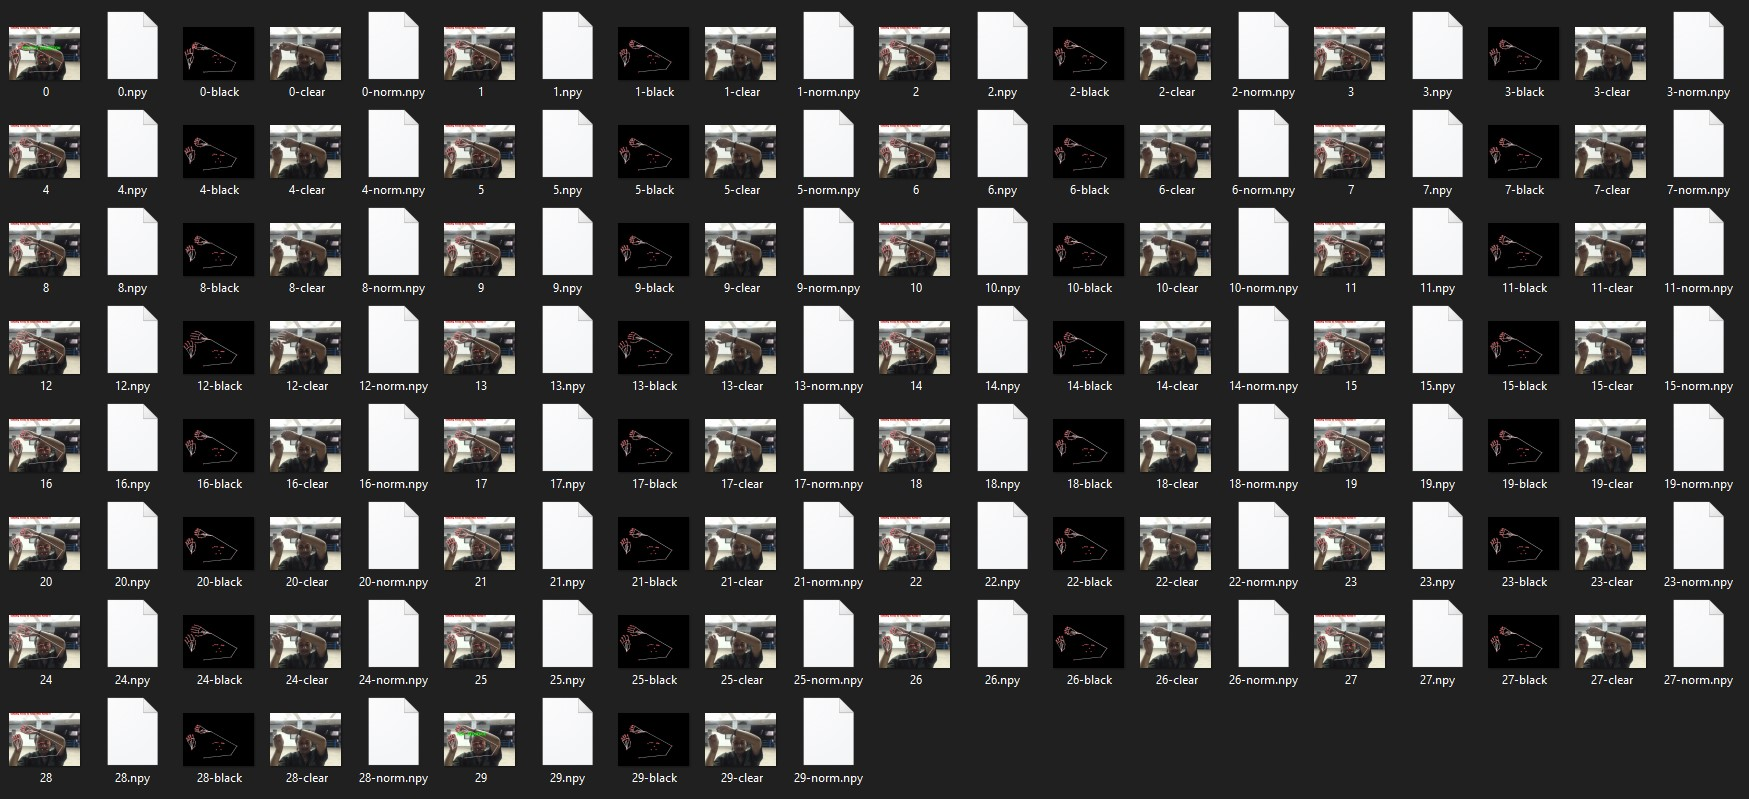
\includegraphics[scale=0.28]{gambar/dataset.jpg}
  % Keterangan gambar yang diinputkan
  \caption{Dataset untuk gestur kanan}
  % Label referensi dari gambar yang diinputkan
  \label{fig:gestur dataset}
\end{figure}

Data citra kedua merupakan input YOLO untuk mendeteksi objek yang ada di depan kursi roda. Data citra ini akan digunakan untuk pendeteksian objek penghalang di depan kursi roda yang berguna untuk \emph{braking system} dari kursi roda
\begin{figure} [H] \centering
  % Nama dari file gambar yang diinputkan
  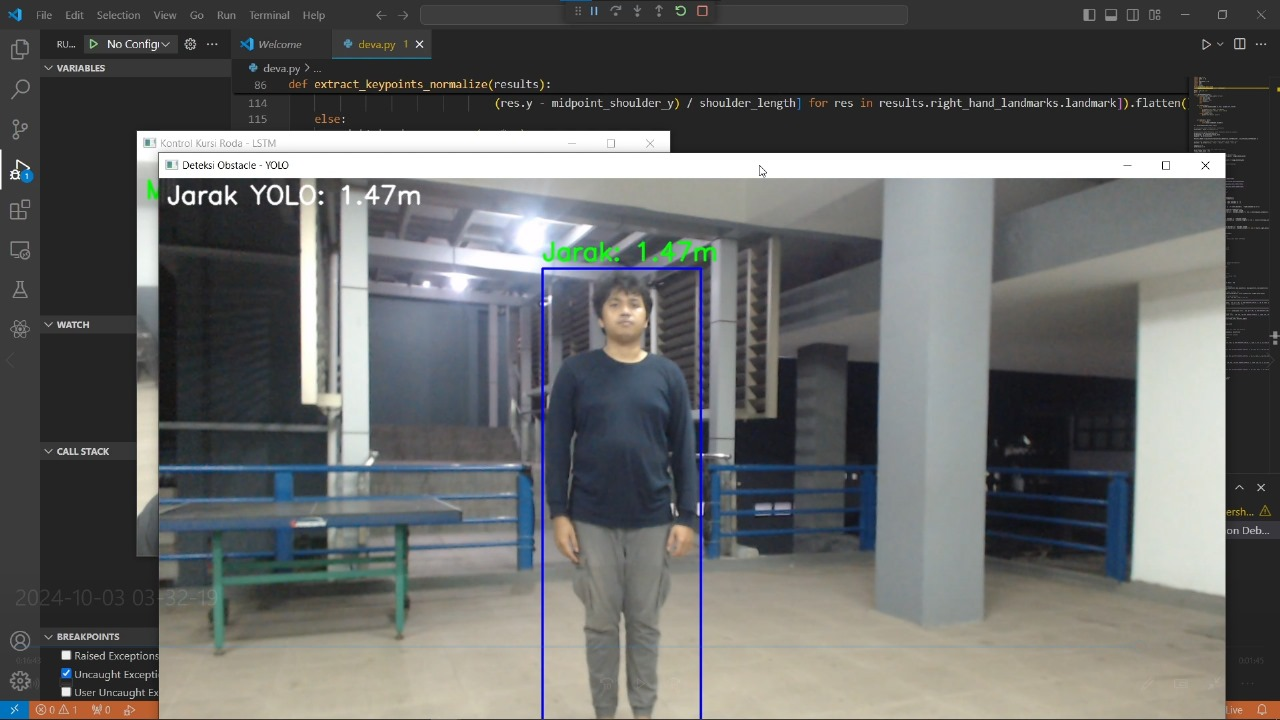
\includegraphics[scale=0.35]{gambar/yolo.jpg}
  % Keterangan gambar yang diinputkan
  \caption{Hasil deteksi YOLO}
  % Label referensi dari gambar yang diinputkan
  \label{fig:citra yolo}
\end{figure}

\subsection{Ekstraksi Fitur}
Ekstraksi fitur dalam program LSTM (Long Short-Term Memory) adalah proses pengambilan informasi penting dari data mentah untuk digunakan sebagai input bagi model. Proses ini bertujuan untuk menyederhanakan data dan menyoroti pola atau karakteristik relevan yang dapat membantu model memahami hubungan temporal dalam data berurutan seperti teks, sinyal, atau deret waktu. Metode ekstraksi fitur bisa dilakukan secara manual, misalnya dengan menghitung statistik dasar seperti rata-rata atau transformasi sinyal seperti FFT, atau secara otomatis menggunakan model pembelajaran mendalam untuk menghasilkan representasi numerik, seperti word embeddings untuk teks atau representasi vektor dari gambar. Dalam konteks LSTM, fitur-fitur yang telah diekstraksi ini diorganisasi dalam urutan yang sesuai dengan waktu atau konteks data, sehingga LSTM dapat mempelajari hubungan temporal antar fitur secara efektif. Dengan ekstraksi fitur yang tepat, model LSTM dapat bekerja lebih efisien, menghasilkan kinerja yang lebih baik dengan memanfaatkan informasi relevan dan mengurangi gangguan dari data mentah.

\subsection{Normalisasi}
Normalisasi adalah proses transformasi data untuk menyelaraskan nilai-nilainya dalam rentang tertentu atau membuat distribusinya konsisten, sehingga mempermudah analisis dan meningkatkan kinerja model pembelajaran mesin. Proses ini bertujuan untuk mengurangi pengaruh skala fitur yang besar terhadap model, mempercepat konvergensi selama pelatihan, dan mencegah dominasi fitur tertentu. Metode normalisasi yang umum meliputi Min-Max Scaling, yang mengubah nilai ke rentang tertentu seperti 0 hingga 1, dan Z-Score Normalization, yang menyelaraskan data sehingga memiliki rata-rata 0 dan standar deviasi 1. Misalnya, dalam citra digital, normalisasi dilakukan dengan mengubah nilai piksel dari skala 0-255 menjadi 0 hingga 1 agar lebih mudah diproses oleh model. Dengan normalisasi, semua fitur dalam data berada pada skala yang seimbang, memungkinkan algoritma pembelajaran mesin untuk lebih fokus pada pola dan hubungan dalam data tanpa terganggu oleh perbedaan skala antar fitur.

\subsection{Klasifikasi Gestur}
Pada tahap ini, gestur yang sudah diambil selanjutnya diklasifikasikan sesuai dengan perintah yang ada pada kursi roda. Terdapat 5 kelas yang digunakan yang kelas maju, kelas mundur, kelas kanan, kelas kiri, dan kelas stop.

\subsection{Braking System}
Klasifikasi dari YOLO nantinya akan digunakan untuk melakukan \emph{braking} otomatis jika mendeteksi kelas yang ditentukan, dalam penelitian ini kelas yang digunakan adalah manusia. Jarak untuk menentukan \emph{braking} adalah 1.3 meter. Jika dalam jarak 1.3 meter terdeteksi manusia maka kursi roda akan berhenti secara otomatis, ini berguna untuk mengurangi resiko kecelakaan pengguna kursi roda.
\subsection{Motion Command}
Motion command adalah perintah yang digunakan untuk mengendalikan gerakan suatu objek atau perangkat, seperti kursi roda, dengan memberikan instruksi terkait arah, kecepatan, atau posisi yang harus dicapai. Dalam konteks penelitian ini, motion command berfungsi untuk mengubah input gestur menjadi perintah gerakan yang spesifik untuk kursi roda. Setiap kelas yang Anda gunakan (A, B, C, D, dan E) mewakili jenis perintah gerakan yang berbeda: Kelas A untuk bergerak ke kiri, kelas B untuk bergerak maju, kelas C untuk berhenti, kelas D untuk bergerak mundur, dan kelas E untuk bergerak ke kanan. Setelah sistem mendeteksi gestur yang sesuai, seperti gerakan tangan atau tubuh, hasil klasifikasi tersebut diterjemahkan menjadi motion command yang dikirim ke sistem kendali kursi roda. Perintah ini kemudian dieksekusi oleh motor atau aktuator kursi roda untuk melaksanakan gerakan yang diinginkan. Dengan menggunakan motion command yang terhubung langsung ke kelas gestur, sistem dapat mengendalikan kursi roda secara responsif dan akurat berdasarkan input dari pengguna.

\subsection{Motion Planning}
Motion planning adalah proses perencanaan jalur atau gerakan bagi suatu objek atau perangkat untuk mencapai tujuan tertentu dengan mempertimbangkan berbagai faktor, seperti hambatan, batasan kecepatan, dan kondisi lingkungan. Dalam konteks robotika atau kendaraan otonom, motion planning bertujuan untuk merencanakan serangkaian langkah atau aksi yang harus diambil agar objek dapat bergerak dari titik awal menuju titik tujuan secara aman, efisien, dan sesuai dengan batasan yang ada. Proses ini melibatkan pembuatan peta lingkungan yang menggambarkan hambatan yang harus dihindari, serta perencanaan jalur yang menghubungkan posisi awal dan tujuan. Selain itu, motion planning juga mencakup optimasi jalur untuk meningkatkan efisiensi, seperti mengurangi waktu atau energi yang dibutuhkan, dan eksekusi jalur tersebut dengan mengontrol perangkat untuk mengikuti rute yang telah direncanakan. Dalam kendaraan otonom, misalnya, motion planning digunakan untuk merencanakan jalur yang menghindari kendaraan lain dan rintangan di jalan, sementara dalam robotika, motion planning memastikan robot dapat bergerak dari satu lokasi ke lokasi lain tanpa menabrak objek sekitarnya. Dengan demikian, motion planning memungkinkan perangkat bergerak secara cerdas, aman, dan responsif terhadap lingkungan sekitarnya.

\newpage
\subsection{Training Model}
Pada tahap ini, dataset yang sudah diklasifikasi selanjutnya akan masuk ke tahap training ke sel LSTM.
\begin{figure} [H] \centering
  % Nama dari file gambar yang diinputkan
  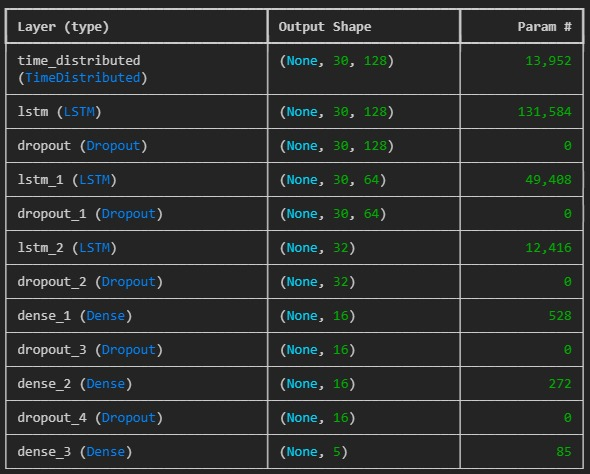
\includegraphics[scale=0.6]{gambar/training model.jpg}
  % Keterangan gambar yang diinputkan
  \caption{Struktur LSTM untuk Training Gestur Tangan}
  % Label referensi dari gambar yang diinputkan
  \label{fig:training model}
\end{figure}
Proses dimulai dengan lapisan TimeDistributed, yang menerapkan transformasi pada setiap langkah waktu dari data sekuensial dengan panjang 30, menghasilkan keluaran dengan dimensi 128. Lapisan ini digunakan untuk mengolah data dengan fitur per frame, seperti hasil dari pose estimation. Selanjutnya, lapisan LSTM pertama memproses data sekuensial untuk menangkap pola temporal dengan keluaran 128 per langkah waktu, diikuti dengan lapisan Dropout untuk mencegah overfitting. Lapisan LSTM kedua mengurangi dimensi keluaran menjadi 64 unit untuk fokus pada pola yang lebih signifikan, diikuti oleh Dropout kedua. LSTM ketiga mengurangi dimensi menjadi 32 unit untuk mempertahankan informasi penting, dengan Dropout ketiga untuk menjaga generalisasi. Setelah itu, lapisan Dense pertama mengintegrasikan informasi dari lapisan sebelumnya dengan 16 unit, diikuti dengan Dropout untuk regularisasi. Lapisan Dense kedua juga memiliki 16 unit untuk memperdalam pengolahan informasi, disertai dengan Dropout keempat. Lapisan Dense ketiga, yang merupakan lapisan output, menghasilkan 5 neuron yang kemungkinan mewakili 5 kelas gestur atau tindakan berbeda. Dengan penggunaan Dropout di setiap tahap, model ini dirancang untuk mencegah overfitting dan meningkatkan generalisasi agar dapat bekerja dengan baik pada data baru.

\newpage
\section{Hardware}
pada tahap ini, perancangan hardware dilakukan sesuai dengan alur yang telah direncanakan sebelumnya. Perancangan ini akan dipresentasikan dengan blok diagram alur yang telah mereprentasikan alur dari bagian hardware.
\begin{figure} [H] \centering
  % Nama dari file gambar yang diinputkan
  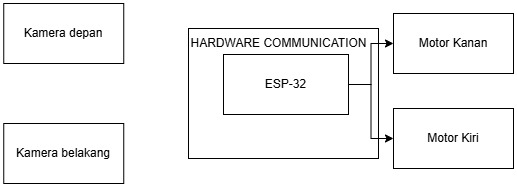
\includegraphics[scale=0.6]{gambar/hardware new.jpg}
  % Keterangan gambar yang diinputkan
  \caption{Diagram Hardware}
  % Label referensi dari gambar yang diinputkan
  \label{fig:hardware}
\end{figure}

\subsection{Kamera Depan}
Kamera depan berfungsi sebagai hardware untuk mengambil citra untuk YOLO yang akan mendeteksi objek manusia. Setelah citra diproses, YOLO akan membagi gambar menjadi grid dan menghasilkan prediksi berupa bounding box, label kelas, dan skor probabilitas untuk setiap objek yang terdeteksi. Dengan cara ini, kursi roda atau sistem dapat mengidentifikasi objek di jalur depan dan berhenti ketika mendeteksi manusia. Kamera depan berfungsi sebagai "mata" sistem untuk memberikan informasi visual yang diperlukan bagi YOLO untuk melakukan deteksi objek secara real-time.

\subsection{Kamera Belakang}
Kamera belakang berfungsi sebagai input citra untuk LSTM. Prosesnya dimulai dengan kamera belakang yang menangkap citra atau video dari pengguna kursi roda. MediaPipe akan menganalisis citra tersebut dan mendeteksi landmark tubuh, misalnya posisi tangan yang kemudian diterjemahkan menjadi input untuk model LSTM. LSTM akan memproses urutan data ini, memahami pola gerakan atau posisi tubuh pengguna, dan menghasilkan output yang sesuai, seperti perintah untuk menggerakkan kursi roda maju, mundur, atau berbelok. Dengan menggunakan LSTM, model dapat mengingat dan merespons gerakan tubuh sebelumnya, memberikan kontrol yang lebih lancar dan alami atas kursi roda, berdasarkan input gestur atau posisi tubuh yang terdeteksi oleh kamera belakang.
\subsection{Laptop}
Pada tahap awal, data di peroleh dengan menggunakan kamera yang dipasang pada bracket khusus. Desain bracket ini memungkinkan kamera untuk menangkap citra tangan dengan sudut pandang yang optimal, sehingga memastikan pengambilan gambar yang akurat. Proses ini melibatkan pengambilan gambar dan video secara real-time, yang sangat penting untuk memastikan data yang dihasilkan relevan dan dapat digunakan untuk analisis lebih lanjut.

Setelah citra berhasil dikumpulkan, langkah berikutnya adalah pengolahan data tersebut dengan melakukan klasifikasi menggunakan Model LSTM yang telah dilatih sebelumnya, yang disimpan dalam format .h5. Model ini digunakan untuk mendeteksi gestur yang terdeteksi dalam citra. Untuk mendukung proses ini, beberapa library perlu diinstal terlebih dahulu, dan instalasinya dilakukan melalui serangkaian perintah yang telah ditentukan. Adapun penggunaan library yang akan digunakan ialah, Mediapipe, Scikit - learn, tensor-
flow, keras, seaborn, numpy dan opencv-python. Library - library ini memastikan semua alat dan dependensi yang diperlukan untuk menjalankan model tersebut pada perangkat laptop.

Spesifikasi laptop yang digunakan dalam penelitian ini adalah laptop ROG Strix G512LU dengan spesifikasi sebagai Tabel berikut:
\begin{table}[ht]
\centering
\begin{tabular}{|c|c|}
\hline
\textbf{Spesifikasi} & \textbf{Detail} \\ \hline
CPU & Intel Core I7-10750H \\ \hline
RAM & 16 GB DDR4\\ \hline
GPU & GTX 1660 Ti \\ \hline
\end{tabular}
\caption{Spesifikasi Laptop}
\label{tab:spec_laptop}
\end{table}
Pada tugas akhir ini, data citra tangan yang telah diproses dan diklasifikasikan akan menghasilkan perintah yang dikirimkan dari laptop ke ESP32 melalui koneksi WiFi. Pengiriman data ini sangat penting karena hasil klasifikasi akan digunakan untuk mengendalikan motor pada kursi roda, memungkinkan kursi roda dikendalikan melalui gestur tangan.

Untuk memastikan pengiriman data berjalan lancar, laptop harus terlebih dahulu terhubung ke access point yang disediakan oleh ESP32. Proses ini melibatkan konfigurasi koneksi WiFi pada laptop agar dapat berkomunikasi dengan ESP32. Setelah koneksi berhasil, data klasifikasi mulai dikirim. Pengiriman data dilakukan menggunakan bahasa pemrograman Python, yang dipilih karena fleksibilitasnya dalam menangani operasi jaringan dan pengolahan data. Data dikirim dalam format string, yang sederhana namun efektif untuk transmisi data melalui jaringan.

Untuk membangun koneksi jaringan yang memungkinkan pengiriman dan penerimaan data, digunakan beberapa library Python seperti socket, time, dan datetime. Library socket menangani komunikasi jaringan, memungkinkan program untuk mengirim dan menerima data melalui koneksi TCP/IP. Library time digunakan untuk mengatur interval pengiriman data, memastikan data dikirim pada waktu yang tepat. Sementara itu, library datetime mencatat waktu pengiriman data untuk keperluan logging dan debugging.

IP Address dari access point ESP32 digunakan sebagai variabel host dalam program, sementara port 80 digunakan sebagai variabel port. Port 80 adalah port standar untuk komunikasi HTTP, yang memungkinkan penggunaan protokol HTTP untuk pengiriman data. Setelah semua konfigurasi selesai, program akan menghubungkan ke server sesuai dengan IP Address dan port yang telah ditentukan, memastikan pengiriman data dari laptop ke ESP32 berjalan dengan lancar.Program ini dirancang untuk berjalan secara terus-menerus, menerima input dari pengguna dan mengirimkan data ke ESP32 tanpa batas waktu.

\subsection{ESP-32}
Pada ESP-32 akan menerima data dari laptop untuk memberikan perintah pada kursi roda sesuai dengan kelas yang dipanggil secara \emph{real-time}. Program dimulai dengan mengimpor beberapa library yang diperlukan untuk menjalankan berbagai fungsi, seperti WiFi, Arduino, dan JSON. Library WiFi digunakan untuk mengelola koneksi jaringan, library Arduino untuk mengontrol perangkat keras, dan library JSON untuk memproses data dalam format JSON. Setelah itu, dilakukan inisialisasi pada komunikasi serial, WiFi, dan server untuk memastikan bahwa ESP32 siap menerima dan mengirimkan data melalui jaringan.

Selanjutnya, program memeriksa apakah ada perangkat yang terhubung ke server ESP32 dengan menggunakan fungsi pemeriksa koneksi jaringan. Jika tidak ada perangkat yang terhubung, program akan terus memeriksa hingga perangkat berhasil terhubung. Setelah perangkat terhubung, program akan memeriksa apakah ada data yang dikirimkan. Jika ada data yang diterima, program akan masuk ke dalam loop untuk membaca data secara terus-menerus. Data yang diterima kemudian akan disimpan dalam variabel \texttt{receivedData}, dan string data akan dibaca hingga ditemukan karakter newline (/n), yang menandakan akhir dari data tersebut.
Setelah data diterima dan disimpan, string data tersebut akan diekstraksi untuk mendapatkan informasi mengenai arah dan kecepatan. Proses ekstraksi ini sangat penting untuk mengonversi string data menjadi format yang dapat digunakan oleh program untuk mengendalikan motor pada kursi roda. Setelah ekstraksi selesai, data arah dan kecepatan yang telah diproses akan ditampilkan guna memastikan bahwa informasi yang diterima sesuai dengan yang diharapkan. Dengan data arah dan kecepatan yang sudah tersedia, ESP32 dapat mengirimkan instruksi ke motor kursi roda agar bergerak sesuai dengan perintah yang diterima. Proses ini akan terus berulang selama perangkat tetap terhubung dan data terus diterima. Berikut merupakan perintah sesuai dengan kelas yang dipanggil:

\begin{table}[H]
    \centering
    \begin{tabular}{|c|c|}
    \hline
    \textbf{Klasifikasi gestur} & \textbf{Kode Intruksi} \\ \hline
    Kiri & A \\ \hline
    Maju & B \\ \hline
    Stop & C \\ \hline
    Mundur & D \\ \hline
    Kanan & E \\ \hline
    \end{tabular}
    \caption{Kode Instruksi dari hasil klasifikasi}
    \label{tab:kode intruksi}
\end{table}

Sesuai dengan Tabel 3.2, kode intruksi tersebut diimplementasikan dengan hasil gestur yang didapatkan dari hasil training LSTM. Pengoperasian dari kursi roda diawali dengan intruksi kode B yakni maju, jika pengguna mengintruksikan kode A atau E kursi roda akan berbelok ke kiri atau kanan. Namun perlu diperhatikan, apabila ingin berganti arah agar motor tidak mengalami kesalahan dalam menerima input yang dihasilkan model, maka perlu dilakukan pemanggilan kelas ’Stop’ atau mengirim instruksi ’C’.

\newpage
\subsection{Skematik Alat}
\begin{figure} [H] \centering
  % Nama dari file gambar yang diinputkan
  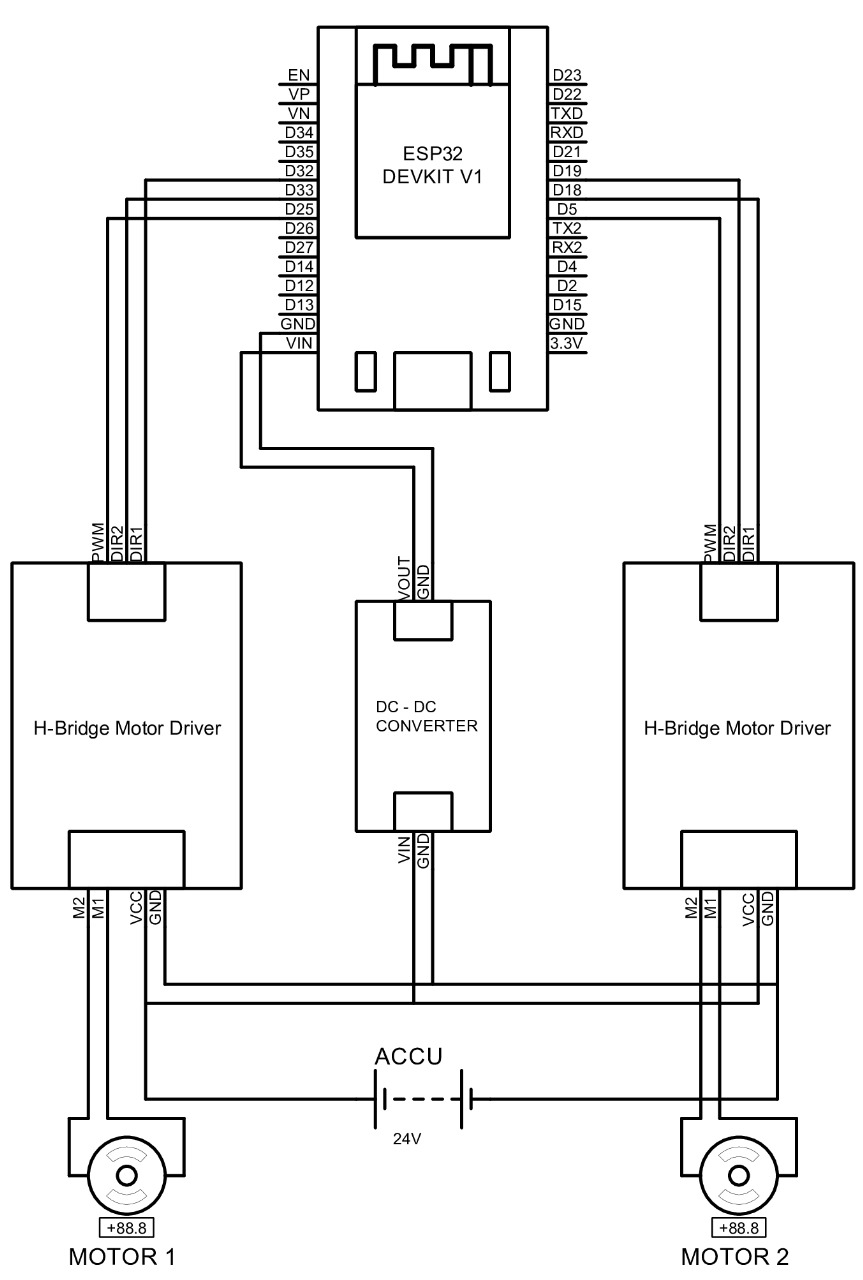
\includegraphics[scale=0.4]{gambar/skematik alat.jpg}
  % Keterangan gambar yang diinputkan
  \caption{Skematik kontrol motor kursi roda\cite{ekatama2024perancangan}}
  % Label referensi dari gambar yang diinputkan
  \label{fig:skematik kontrol}
\end{figure}

Dari penelitian yang telah dilakukan, telah dirancang sebuah sistem kontrol untuk motor
kursi roda dengan skematik alat yang ditampilkan pada Gambar 3.8. ESP32 akan terhubung
dengan dua buah H-Bridge Motor Driver dan sebuah DC-DC Converter. Setiap H-Bridge Mo-
tor Driver terhubung langsung ke motor roda kiri dan motor roda kanan untuk menggerakkan
roda kursi roda secara efektif. Dalam skematik ini, ESP32 berfungsi sebagai otak dari sistem, mengirimkan sinyal kontrol ke motor driver berdasarkan data yang diterima melalui koneksi WiFi\cite{ekatama2024perancangan}.

 Program dirancang untuk mengendalikan motor DC dengan memproses perintah yang dikirim melalui jaringan WiFi. Tahapan pertama dalam program adalah mengimpor library yang dibutuhkan, seperti Arduino dan WiFi, untuk menyediakan fungsi-fungsi penting. Setelah itu, dilakukan inisialisasi PWM dan konfigurasi pin sebagai saluran untuk mengirim sinyal kontrol ke motor driver.

Setelah inisialisasi selesai, program mulai memeriksa koneksi dengan perangkat yang terhubung ke server ESP32. Jika belum ada perangkat yang terhubung, program akan terus memantau hingga koneksi berhasil. Ketika koneksi berhasil, program melanjutkan dengan memeriksa apakah ada data yang diterima dari perangkat tersebut. Jika data ditemukan, program membacanya hingga mendeteksi karakter newline (/n), yang menunjukkan akhir dari string data.

Data yang diterima selanjutnya diproses untuk mengekstrak informasi mengenai arah dan kecepatan. Tahap ini mengubah string data menjadi format yang dapat digunakan oleh program untuk mengontrol motor kursi roda. Berdasarkan informasi ini, ESP32 mengirimkan instruksi ke motor driver untuk menggerakkan roda sesuai arah dan kecepatan yang diinginkan.

Sistem kontrol kursi roda ini menggunakan dua metode pengendalian. Metode pertama adalah differential drive, di mana roda kanan bergerak mundur dan roda kiri maju saat berbelok ke kanan, serta sebaliknya untuk berbelok ke kiri. Metode kedua adalah gerakan normal, di mana roda kanan diam dan roda kiri bergerak maju saat berbelok ke kanan, atau sebaliknya saat berbelok ke kiri. Saat bergerak maju atau mundur, kedua roda berputar serentak ke arah yang sama. Dalam penelitian ini, metode kedua dipilih untuk mengendalikan pergerakan kursi roda.

Program ini memastikan ESP32 dapat berfungsi secara optimal sebagai pengontrol motor. Setiap langkah dalam flowchart dirancang untuk memastikan sistem bekerja dengan efisien dan responsif terhadap perintah yang diterima melalui jaringan WiFi. Dengan pengoperasian secara real-time, sistem mampu merespons perintah dengan cepat dan memberikan kontrol yang presisi untuk pergerakan kursi roda\cite{ekatama2024perancangan}.